\section{Evaluación de los modelos en HealthBench}
\label{sec:evaluacion-healthbench}
\label{sec:protocolo-experimental}
\label{sec:evaluacion-protocolo}
\subsection{Modelos evaluados}
Las variantes consideradas fueron Qwen2.5-7B Base~\cite{qwen2024qwen25}, como referencia sin adaptación al dominio, Qwen2.5-7B SFT-70, adaptado con la partición del 70\%, y Qwen2.5-7B SFT-90, adaptado con la partición del 90\%. A partir de esta última variante se evaluó el experimento central con GRPO, que incorporó las rúbricas, la recompensa híbrida y la retirada progresiva de ayudas descritas en el capítulo~\ref{ch:metodo-propuesto}. En adelante se lo identifica como SFT-90 + GRPO, mientras que el identificador V23 se conserva únicamente para vincularlo con los archivos del experimento.

La comparación cuantitativa se limitó a SFT-90 y SFT-90 + GRPO, cuyas evaluaciones cubrieron los mismos 500 casos y 5.739 criterios, bajo las condiciones descritas en la sección~\ref{sec:protocolo-experimental}. Por su parte, Base y SFT-70 quedaron como antecedentes experimentales, ya que los archivos de evaluación disponibles no permitieron construir una comparación completa y equivalente con esos modelos.

\subsection{Conjunto de evaluación externa}
Los experimentos centrales utilizan un subconjunto fijo de 500 casos de la versión general, denominado operativamente HealthBench-500, que contiene 5.739 criterios compartidos por las evaluaciones de SFT y GRPO. Esta denominación identifica la muestra del proyecto y no una variante oficial adicional.

\subsection{Condiciones de generación}
Para que la comparación sea interpretable, deben conservarse los casos, la plantilla de conversación y las condiciones de generación, registrando el checkpoint y la configuración de cada modelo. En los experimentos centrales, los manifiestos de generación declaran respuestas deterministas con temperatura $0{,}0$ y muestreo desactivado (\texttt{do\_sample = False}), un límite máximo de 512 tokens nuevos (\texttt{max\_new\_tokens = 512}) y carga del modelo en precisión \texttt{bfloat16}. Sin embargo, compartir esos parámetros no basta para acreditar igualdad de condiciones, ya que también deben documentarse el tokenizador, las versiones del software y cualquier diferencia en el procesamiento de las entradas. Asimismo, la comparación con el modelo base requiere completar y auditar su evaluación antes de incorporarlo a una tabla conjunta.

\subsection{Modelo juez y control de las evaluaciones}
Las evaluaciones disponibles utilizan un juez local identificado en los registros como Qwen3.8-27B, desplegado sobre el motor de inferencia vLLM~\cite{kwon2023vllm} en una instancia distribuida. El servicio se ejecutó bajo cuantización FP8 (8-bit en punto flotante, registrado en los metadatos con la etiqueta \texttt{qwen3.8-27b-judge-8bit}), descartando cuantizaciones más agresivas (como INT4) para mitigar la degradación en la fidelidad de la interpretación semántica. El evaluador operó con una ventana de contexto de 4.096 tokens (\texttt{max-model-len = 4096}), un presupuesto de salida de hasta 1.024 tokens con cadena de razonamiento habilitada y decodificación determinista con temperatura $0{,}0$. Al emplearse un juez local desplegado en vLLM en lugar del protocolo original de OpenAI (que recurre a modelos de frontera comerciales vía API), los resultados se describen como evaluaciones sobre HealthBench con juez local, sin asumir equivalencia numérica directa con las cifras reportadas en la literatura por OpenAI~\cite{arora2025healthbench}.

Antes de calcular las métricas se comprueba que cada identificador tenga una única respuesta y que todos sus criterios dispongan de una decisión válida. La auditoría de los archivos finales de los experimentos centrales confirma 500 casos y 5.739 decisiones por modelo, sin criterios faltantes, adicionales o duplicados y con coincidencia en el texto, los pesos y las etiquetas de los criterios. Un fallo del juez debe registrarse como pendiente o fallido, porque interpretarlo como incumplimiento introduciría una penalización ajena a la respuesta. Por ello, también se conservan los reintentos, los errores y cualquier reparación aplicada al formato de salida.

La cobertura completa debe distinguirse de la homogeneidad experimental. En la evaluación de SFT se utilizaron varios servidores y faltan metadatos que permitan identificar el modelo juez en todas las decisiones, mientras que el experimento GRPO conserva su etiqueta de modelo. Además, 26 decisiones de SFT se incorporaron a partir del valor booleano guardado aunque la salida original no conservara un JSON final estricto. Estas diferencias limitan la atribución causal al entrenamiento y requieren recalificar ambos conjuntos con un único checkpoint, prompt y procedimiento de lectura del juez para obtener una comparación homogénea.


\subsection{Cambios por dimensiones y cumplimiento de criterios}
\label{sec:resultados-dimensiones}

Los resultados de esta sección corresponden exclusivamente a Qwen2.5-7B SFT-90 y SFT-90 + GRPO de la primera etapa. Su propósito es evaluar el comportamiento de la integración inicial y orientar las decisiones metodológicas posteriores.

El análisis distinguió los criterios individuales, evaluados mediante decisiones de cumplimiento, de los ejes que agruparon esos criterios. En los cuatro ejes presentados, la precisión se relacionó con la corrección de la información, la comunicación con su claridad y adecuación, la comprensión del contexto con el uso de los antecedentes disponibles y el seguimiento de instrucciones con las condiciones solicitadas. Estas dimensiones se interpretaron como desgloses descriptivos del benchmark y no como métricas oficiales adicionales~\cite{arora2025healthbench}.

Para cada eje se aplicó el procedimiento descrito en la ecuación~\ref{eq:healthbench-ejes}: se sumaron los pesos de los criterios cumplidos en cada caso, incluidos los negativos, y se normalizaron por los puntos positivos posibles de ese eje. Luego se promediaron los casos con denominador positivo y se recortó la media al intervalo de 0 a 1. Por ello, las puntuaciones de la tabla~\ref{tab:resultados-ejes} no representaron el porcentaje simple de criterios cumplidos. La cantidad de casos incluidos varió entre ejes, aunque fue idéntica para ambos modelos dentro de cada comparación.

\begin{table}[htbp]
\centering
\caption{Comparación descriptiva por ejes de HealthBench.}
\label{tab:resultados-ejes}
\begin{tabularx}{\textwidth}{@{}Ccccc@{}}
\toprule
Eje & SFT-90 & SFT + GRPO & Diferencia & Casos \\
\midrule
Precisión & 6,41\% & 7,80\% & $+1,39$ pp & 421 \\
Calidad de comunicación & 17,08\% & 12,97\% & $-4,11$ pp & 217 \\
Comprensión del contexto & 4,67\% & 8,33\% & $+3,66$ pp & 327 \\
Seguimiento de instrucciones & 6,79\% & 11,37\% & $+4,58$ pp & 93 \\
\bottomrule
\end{tabularx}
\end{table}

El modelo optimizado con GRPO obtuvo puntuaciones mayores en seguimiento de instrucciones y comprensión del contexto, con diferencias de 4,58 y 3,66 puntos porcentuales, respectivamente, mientras que la precisión presentó una diferencia de $+1,39$ puntos. Sin embargo, la calidad de comunicación descendió 4,11 puntos porcentuales, por lo que la comparación mostró un comportamiento distinto según la dimensión analizada. La figura~\ref{fig:resultados-ejes} reúne estos resultados, cuyas diferencias se interpretaron descriptivamente y no como evidencia de significancia estadística.

\begin{figure}[htbp]
\centering
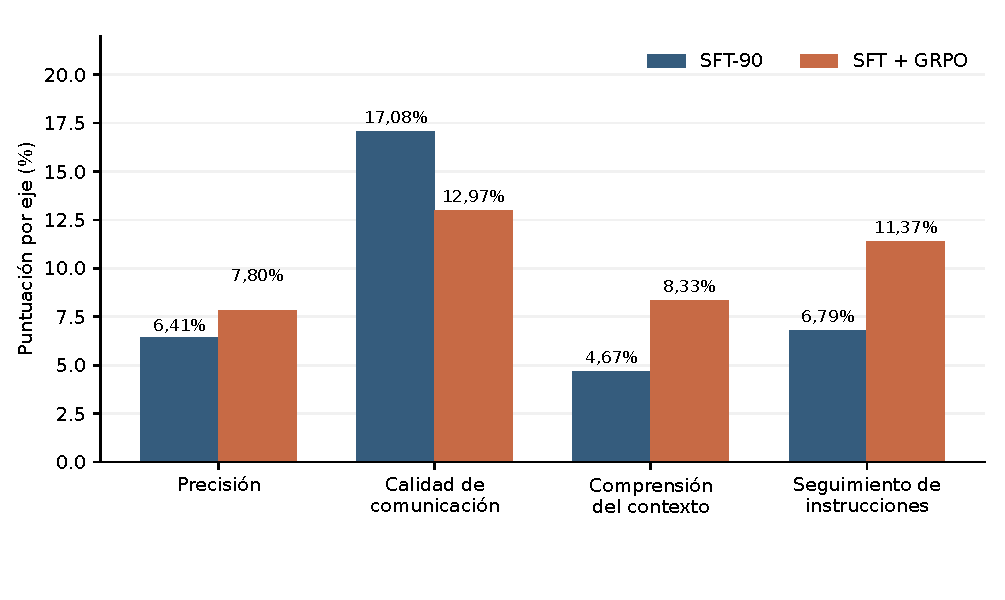
\includegraphics[width=\textwidth]{Figuras/04-resultados/resultados-ejes.pdf}
\caption{Comparación de SFT-90 y SFT-90 + GRPO en cuatro ejes.}
\label{fig:resultados-ejes}
\end{figure}

Como complemento, la tabla~\ref{tab:resultados-criterios} presenta los conteos no ponderados de los criterios positivos cumplidos y de los negativos activados. El modelo con GRPO cumplió 85 criterios positivos más, pero también activó 40 criterios negativos adicionales, de modo que el aumento de cobertura estuvo acompañado por una mayor frecuencia de comportamientos penalizados. Estos últimos incluyeron distintos tipos de errores y no se redujeron exclusivamente a problemas de seguridad clínica.

\begin{table}[htbp]
\centering
\caption{Cumplimiento de criterios sin ponderación por sus pesos.}
\label{tab:resultados-criterios}
\begin{tabularx}{\textwidth}{@{}Ccc@{}}
\toprule
Medida & SFT-90 & SFT-90 + GRPO \\
\midrule
Criterios positivos cumplidos & 626/4.003 & 711/4.003 \\
Proporción de positivos cumplidos & 15,64\% & 17,76\% \\
Criterios negativos activados & 672/1.736 & 712/1.736 \\
Proporción de negativos activados & 38,71\% & 41,01\% \\
\bottomrule
\end{tabularx}
\end{table}

La figura~\ref{fig:resultados-criterios} representa esas proporciones por separado, porque utilizaron denominadores distintos. Por tanto, no se sumaron como una puntuación única ni se equipararon con los resultados ponderados de los ejes, donde un criterio de mayor peso tuvo una contribución diferente de otro con menor peso.

\begin{figure}[htbp]
\centering
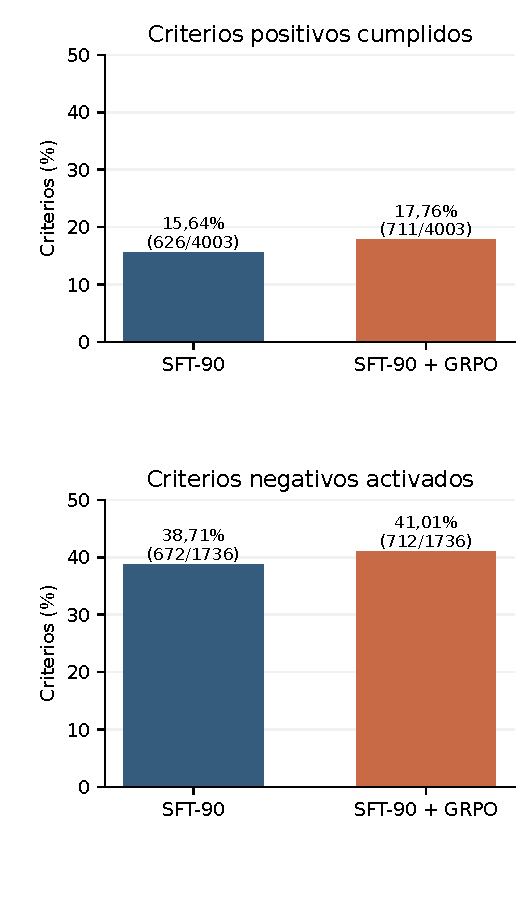
\includegraphics[width=8.9cm]{Figuras/04-resultados/resultados-criterios.pdf}
\caption{Criterios positivos cumplidos y negativos activados.}
\label{fig:resultados-criterios}
\end{figure}
